% =====================================================================
% Guía del estudiante -- Cálculo 11° -- Trimestre I
% María Mercedes Cantillo · Colegio San Alberto Magno
% ---------------------------------------------------------------------
% Plan: materias/calculo/undecimo/curriculo/plan-anual.md y filas 001-036
% de programacion.csv. Cada \tema tiene \label{tema:...} para que las
% clases lo citen con \refguia{tema:...}. No borrar el .aux de esta guía.
%
% Compilar:  latexmk -pdf guia-periodo-I-numeros-reales.tex
% =====================================================================
\documentclass[11pt]{article}
\makeatletter\def\input@path{{../../../../plantillas/estilo/}}\makeatother
\usepackage{mmcantillo}

% ======================== DATOS DE LA GUÍA ============================
\tipodocumento{Guía del estudiante}
\asignatura{Cálculo}
\titulo{Los números reales: orden e infinito}
\grado{11°}
\periodo{I}
\hiloconductor{La historia del infinito}
% ======================================================================
% DBA: matematicas grado 11 · DBA 1 — Utiliza las propiedades de los números
%      (naturales, enteros, racionales y reales) y sus relaciones y operaciones...
%      DBA 2 — Justifica la validez de las propiedades de orden de los números
%      reales y las utiliza para resolver problemas analíticos que se modelen
%      con inecuaciones.

% Recta numérica para representar intervalos:
%   \abierto{x} / \cerrado{x}: extremo sin / con el punto
\newcommand{\abierto}[1]{\draw[thick, fill=white] (#1,0) circle (3pt);}
\newcommand{\cerrado}[1]{\fill (#1,0) circle (3pt);}

\begin{document}

\encabezado

% ---------------------------------------------------------------------
% 1. Frase introductoria
% ---------------------------------------------------------------------
% verificado: http://www.sur-gmbh.ch/private/burki/Studies/cantor.pdf — «denn das Wesen der Mathematik liegt gerade in ihrer Freiheit», Grundlagen (1883), §8; Gesammelte Abhandlungen, p. 182
\frase{La esencia de la matemática está precisamente en su libertad.}
{Georg Cantor, \emph{Fundamentos de una teoría general de conjuntos} (1883), §8}

% ---------------------------------------------------------------------
% 2. Introducción
% ---------------------------------------------------------------------
\seccion{Introducción}

El cálculo, que estudiaremos este año, es la matemática del cambio: velocidades,
crecimientos, máximos y mínimos. Pero todo el cálculo descansa sobre una idea que
parece sencilla y no lo es: la \textbf{recta real}, una línea donde cada punto es
un número y no hay huecos. En este primer trimestre construiremos esa recta, la
ordenaremos y aprenderemos a movernos en ella con \textbf{desigualdades},
\textbf{inecuaciones} y \textbf{valor absoluto}. Son también herramientas que la
prueba Saber 11 evalúa en todos sus cuadernillos.

Nuestro hilo conductor es una de las aventuras más largas del pensamiento humano:
\emph{la historia del infinito}. Empieza hace 2\,500 años con una hermandad griega
convencida de que todo en el universo podía contarse con números enteros, y termina
a finales del siglo XIX con un matemático que demostró que hay infinitos más
grandes que otros. En el camino encontraremos un secreto que, según la leyenda,
costó una vida; a una filósofa que enseñaba en Alejandría; y a una joven francesa
que tuvo que estudiar con nombre de hombre. Cada tema de esta guía es un paso de
esa historia.

\textbf{Al terminar este trimestre podrás:}
\begin{itemize}
  \item distinguir los sistemas numéricos $\N \subset \Z \subset \Q \subset \R$ y
        explicar por qué cada uno fue necesario;
  \item justificar que existen números irracionales y ubicarlos en la recta real;
  \item escribir conjuntos de números como intervalos y operar con ellos;
  \item usar las propiedades de orden para resolver inecuaciones lineales,
        cuadráticas, racionales y con valor absoluto, y expresar sus soluciones
        como intervalos.
\end{itemize}

Este trimestre trabaja dos Derechos Básicos de Aprendizaje del Ministerio de
Educación Nacional~\cite{mendba}:

\begin{dba}[Grado 11 · DBA 1]
Utiliza las propiedades de los números (naturales, enteros, racionales y reales) y
sus relaciones y operaciones para construir y comparar los distintos sistemas
numéricos.
\end{dba}

\begin{dba}[Grado 11 · DBA 2]
Justifica la validez de las propiedades de orden de los números reales y las
utiliza para resolver problemas analíticos que se modelen con inecuaciones.
\end{dba}

% ---------------------------------------------------------------------
% 3. Marco teórico
% ---------------------------------------------------------------------
\seccion{Marco teórico}

\subsubsection*{«Todo es número»: los pitagóricos}

En el siglo VI a.\,C., en el sur de Italia, Pitágoras de Samos fundó una comunidad
que mezclaba filosofía, música y matemáticas. Según Aristóteles, los pitagóricos
pensaban que los principios de los números eran los principios de todas las
cosas~\cite{aristoteles}: las armonías musicales, los movimientos del cielo y las
formas geométricas debían poder expresarse con números enteros y con razones
entre ellos, es decir, con lo que hoy llamamos números racionales.

\subsubsection*{La crisis de los inconmensurables}

Esa convicción se rompió dentro de la propia escuela. Los griegos descubrieron que
la diagonal de un cuadrado y su lado son \emph{inconmensurables}: no existe una
unidad, por pequeña que sea, que quepa un número entero de veces en ambos. Dicho
en lenguaje moderno, $\sqrt{2}$ no es un número racional. La tradición atribuye el
descubrimiento a Hipaso de Metaponto y cuenta, en una leyenda que no podemos
comprobar, que fue castigado por revelarlo~\cite{kline}. Durante siglos, los
matemáticos griegos trataron las longitudes y los números como cosas distintas
para evitar el problema.

\subsubsection*{Alejandría: Diofanto e Hipatia}

En Alejandría, hacia el siglo III, Diofanto escribió la \emph{Aritmética}, una
colección de problemas resueltos con incógnitas, un paso decisivo hacia el
álgebra. Hacia el año 400, \textbf{Hipatia} enseñaba allí matemáticas, astronomía
y filosofía, y según fuentes antiguas escribió comentarios a la obra de Diofanto.
Es la primera mujer matemática de la que tenemos noticias confiables~\cite{dzielska}.

\subsubsection*{Sophie Germain: estudiar a escondidas}

En la Francia de finales del siglo XVIII, las mujeres no podían estudiar en la
École Polytechnique. \textbf{Sophie Germain} consiguió los apuntes de los cursos y
envió sus trabajos firmando como «Monsieur Le Blanc». Así inició una
correspondencia con Carl Friedrich Gauss, el matemático más importante de su
época, sobre teoría de números. Cuando Gauss descubrió que Le Blanc era una mujer,
le escribió:

% verificado: https://www.unesco.org/en/virtual-science-museum/women-science/sophie-germain — traducción inglesa estándar de la carta del 30 abr. 1807 (original en francés); Bucciarelli y Dworsky (1980), cap. 3, pp. 20–29
\begin{cita}{Carl F. Gauss, carta a Sophie Germain (30 de abril de 1807), trad. propia de la versión inglesa; véase~\cite{bucciarelli}, cap. 3}
Cuando una persona del sexo que, según nuestras costumbres y prejuicios, debe
encontrar infinitamente más dificultades que los hombres para familiarizarse con
estas espinosas investigaciones, logra sin embargo superar esos obstáculos y
penetrar en sus partes más oscuras, entonces sin duda debe tener el valor más
noble, talentos del todo extraordinarios y un genio superior.
\end{cita}

\subsubsection*{Dedekind y la recta sin huecos}

¿Qué es exactamente un número real? Durante siglos se usaron sin una definición
precisa. En 1858, mientras preparaba sus clases de cálculo en Zúrich, Richard
Dedekind decidió resolverlo. En \emph{Continuidad y números irracionales} (1872)
definió cada número real como un «corte» que divide a los racionales en dos
grupos, los menores y los mayores. Así demostró que la recta real es
\emph{continua}: no tiene huecos~\cite{dedekind}.

\subsubsection*{Cantor: infinitos de distinto tamaño}

Entre 1874 y 1891, Georg Cantor demostró algo que parecía absurdo: hay tantos
números pares como números naturales, y tantos racionales como naturales, pero
los números reales son \emph{más} que los naturales. Hay infinitos de distinto
tamaño~\cite{kline}. Muchos matemáticos de su tiempo, como Leopold Kronecker,
rechazaron sus ideas. Décadas después, David Hilbert las defendió así:

% verificado: https://eudml.org/doc/159124 — p. 170: «Aus dem Paradies, das Cantor uns geschaffen, soll uns niemand vertreiben können»
\begin{cita}{David Hilbert, «Sobre el infinito» (1926), p. 170, trad. propia~\cite{hilbert}}
Del paraíso que Cantor creó para nosotros, nadie debe poder expulsarnos.
\end{cita}

Las definiciones y procedimientos de esta guía siguen la presentación usual de
los textos de precálculo~\cite{stewart}. Varios ejemplos, ejercicios y las preguntas
tipo Saber 11 están adaptados de la guía de apoyo de Adriana Quintero
Palomino~\cite{quintero}.

% ---------------------------------------------------------------------
% 4. Temas
% ---------------------------------------------------------------------
\tema{Los sistemas numéricos}\label{tema:sistemas}

\begin{hilo}
Samos, siglo VI a.\,C. Para los pitagóricos, contar era entender el mundo: una
cuerda de lira dividida a la mitad suena una octava más aguda, y la razón $2:1$
explica esa armonía. Todo parecía caber en los números enteros y sus razones.
¿Es cierto?
\end{hilo}

Los números se fueron ampliando cada vez que una operación no tenía respuesta:

\begin{itemize}
  \item \textbf{Naturales} $\N = \{0, 1, 2, 3, \ldots\}$: sirven para contar. Pero
        $3 - 5$ no tiene respuesta en $\N$.
  \item \textbf{Enteros} $\Z = \{\ldots, -2, -1, 0, 1, 2, \ldots\}$: la resta siempre
        es posible. Pero $3 \div 5$ no tiene respuesta en $\Z$.
  \item \textbf{Racionales} $\Q = \left\{ \frac{p}{q} : p, q \in \Z,\ q \neq 0 \right\}$:
        la división (salvo por cero) siempre es posible. Todo racional tiene una
        expresión decimal \emph{finita} o \emph{periódica}.
\end{itemize}

Cada conjunto contiene al anterior: $\N \subset \Z \subset \Q$.

\begin{ejemplo}[Un decimal periódico es una fracción]
Sea $x = 0{,}\overline{12} = 0{,}121212\ldots$ Entonces $100x = 12{,}1212\ldots$, y
al restar: $100x - x = 12$, así que $99x = 12$ y
$x = \dfrac{12}{99} = \dfrac{4}{33}$.
\end{ejemplo}

\begin{aplicacion}[Los números dentro de un computador]
Un computador guarda los números en binario, con una cantidad fija de dígitos.
Por eso los enteros tienen un máximo, y un número tan sencillo como $0{,}1$ no se
puede guardar de forma exacta: en muchos lenguajes de programación, $0{,}1 + 0{,}2$
da $0{,}30000000000000004$. Los programadores que trabajan con dinero usan
enteros (centavos) para evitar ese error.
\end{aplicacion}

\begin{preguntas}
\pregunta Para cada operación, di en qué conjunto más pequeño tiene respuesta:
\begin{opciones*}(4)
  \item $7 - 12$
  \item $\dfrac{-8}{4}$
  \item $\dfrac{2}{3} + \dfrac{1}{6}$
  \item $5 \cdot 9$
\end{opciones*}
\espacio{2.5cm}
\pregunta Escribe como fracción irreducible:
\begin{opciones*}(3)
  \item $0{,}\overline{3}$
  \item $0{,}\overline{45}$
  \item $1{,}2\overline{5}$
\end{opciones*}
\espacio{3cm}
\end{preguntas}

\begin{resumen}
\begin{itemize}
  \item $\N \subset \Z \subset \Q$: cada sistema aparece para que una operación
        (resta, división) siempre tenga respuesta.
  \item Un número es racional si se puede escribir como $\frac{p}{q}$ con
        $p, q$ enteros y $q \neq 0$.
  \item Los racionales son exactamente los decimales finitos o periódicos.
\end{itemize}
\end{resumen}

% ---------------------------------------------------------------------
\tema{Los irracionales y la recta real}\label{tema:irracionales}

\begin{hilo}
Un pitagórico mide la diagonal de un cuadrado de lado 1 y busca la fracción que la
exprese. No la encuentra, y no porque le falte paciencia: esa fracción no existe.
Según la leyenda, Hipaso pagó caro revelar el secreto. Dos mil años después,
Dedekind cerraría la herida construyendo la recta real.
\end{hilo}

\begin{teorema}[$\sqrt{2}$ es irracional]
No existen enteros $p$ y $q$ tales que $\left(\frac{p}{q}\right)^2 = 2$.
\end{teorema}

\emph{Demostración (por contradicción).} Supongamos que $\sqrt{2} = \frac{p}{q}$ con
la fracción irreducible. Entonces $p^2 = 2q^2$, así que $p^2$ es par y, por tanto,
$p$ es par: $p = 2k$. Reemplazando, $4k^2 = 2q^2$, es decir, $q^2 = 2k^2$, y $q$
también es par. Pero entonces $p$ y $q$ tienen el factor común 2, lo que
contradice que la fracción era irreducible. \hfill$\square$

Los números cuya expresión decimal es infinita y \textbf{no periódica} se llaman
\textbf{irracionales} ($\mathbb{I}$): $\sqrt{2}$, $\sqrt{3}$, $\pi$, $e$\ldots\ Los
racionales y los irracionales juntos forman los \textbf{números reales}:
$\R = \Q \cup \mathbb{I}$. Cada número real es un punto de la recta, y cada punto
de la recta es un número real.

\begin{definicion}[Densidad]
Entre dos números reales distintos siempre hay otro número real (de hecho,
infinitos). Por ejemplo, entre $a$ y $b$ está su promedio $\frac{a+b}{2}$.
\end{definicion}

\begin{center}
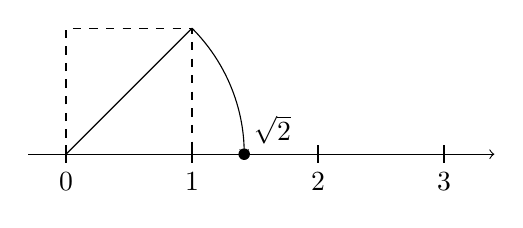
\begin{tikzpicture}[scale=1.6]
  \draw[->] (-0.3,0) -- (3.4,0);
  \foreach \x in {0,1,2,3} \draw (\x,0.07) -- (\x,-0.07) node[below] {$\x$};
  \draw[dashed] (0,0) rectangle (1,1);
  \draw (0,0) -- (1,1);
  \draw[->, thin] (1,1) arc (45:0:1.4142);
  \fill (1.4142,0) circle (1.3pt) node[above right] {$\sqrt{2}$};
\end{tikzpicture}

{\small La diagonal del cuadrado de lado 1 mide $\sqrt{2}$: con un compás la
llevamos a la recta.}
\end{center}

\begin{aplicacion}[La hoja A4]
Las hojas A4, A3, A5\ldots\ tienen una razón entre largo y ancho de
$\sqrt{2} \approx 1{,}414$ (norma internacional ISO 216). Es la única proporción que se
conserva al doblar la hoja por la mitad: por eso una fotocopiadora puede reducir
una hoja A3 a A4 sin deformarla.
\end{aplicacion}

\begin{preguntas}
\pregunta En clase, Carolina dijo: «No entiendo por qué no puedo decir que después
de 5 sigue el 5,1, o el 5,01». Explícale, usando la densidad, por qué ningún
número real es «el siguiente» de 5.
\renglones{3}
\pregunta Escribe tres números racionales y un irracional que estén entre
$0{,}1$ y $0{,}11$.
\espacio{2cm}
\pregunta Adapta la demostración anterior para probar que $\sqrt{3}$ es irracional.
\espacio{3.5cm}
\end{preguntas}

\begin{resumen}
\begin{itemize}
  \item $\sqrt{2}$ no es racional: se demuestra por contradicción.
  \item Irracionales: decimales infinitos no periódicos. $\R = \Q \cup \mathbb{I}$.
  \item La recta real no tiene huecos, y entre dos reales siempre hay infinitos
        reales (densidad): ningún real tiene un «siguiente».
\end{itemize}
\end{resumen}

% ---------------------------------------------------------------------
\tema{Intervalos e infinitos}\label{tema:intervalos}

\begin{hilo}
Berlín, 1874. Georg Cantor se pregunta si todos los infinitos son iguales. Para
compararlos necesita hablar con precisión de «todos los números entre 0 y 1» o
de «todos los mayores que 5». Nace así un lenguaje que usaremos todo el año: los
intervalos.
\end{hilo}

Un \textbf{intervalo} es el conjunto de todos los reales entre dos extremos:

\begin{center}
{\renewcommand{\arraystretch}{1.4}
\begin{tabular}{lll}
  \toprule
  \textbf{Intervalo} & \textbf{Conjunto} & \textbf{Tipo}\\
  \midrule
  $[a, b]$ & $\{x \in \R : a \le x \le b\}$ & cerrado\\
  $(a, b)$ & $\{x \in \R : a < x < b\}$ & abierto\\
  $[a, b)$ & $\{x \in \R : a \le x < b\}$ & semiabierto\\
  $(a, \infty)$ & $\{x \in \R : x > a\}$ & no acotado\\
  $(-\infty, b]$ & $\{x \in \R : x \le b\}$ & no acotado\\
  \bottomrule
\end{tabular}}
\end{center}

El símbolo $\infty$ no es un número: indica que el intervalo no tiene fin. Por eso
siempre va con paréntesis, nunca con corchete.

\begin{ejemplo}[Unión e intersección]
Sean $A = [-2, 3)$ y $B = (1, 5]$. Entonces
$A \cup B = [-2, 5]$ (los que están en al menos uno) y
$A \cap B = (1, 3)$ (los que están en ambos). La \textbf{diferencia} $A - B$ son los
de $A$ que no están en $B$: $A - B = [-2, 1]$. Si dos intervalos no tienen puntos
comunes, su intersección es el conjunto vacío: $(2, 9) \cap (10, \infty) = \varnothing$.

\begin{center}
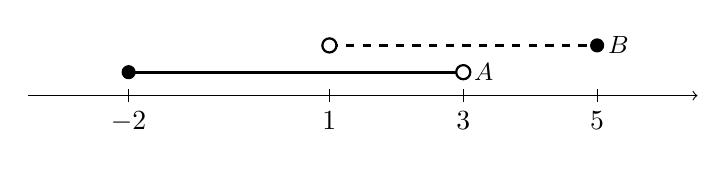
\begin{tikzpicture}[scale=0.85]
  \draw[->] (-3.5,0) -- (6.5,0);
  \foreach \x in {-2,1,3,5} \draw (\x,0.1) -- (\x,-0.1) node[below] {$\x$};
  \draw[very thick] (-2,0.35) -- (3,0.35) node[right] {\small $A$};
  \fill (-2,0.35) circle (3pt); \draw[thick, fill=white] (3,0.35) circle (3pt);
  \draw[very thick, dashed] (1,0.75) -- (5,0.75) node[right] {\small $B$};
  \draw[thick, fill=white] (1,0.75) circle (3pt); \fill (5,0.75) circle (3pt);
\end{tikzpicture}
\end{center}
\end{ejemplo}

\subsubsection*{¿Todos los infinitos son iguales?}

Dos conjuntos tienen el mismo tamaño si sus elementos se pueden emparejar uno a
uno. Los naturales y los pares se emparejan con $n \mapsto 2n$: hay «tantos» pares
como naturales, aunque los pares sean una parte de los naturales. Cantor
demostró que los racionales también se pueden emparejar con los naturales, pero
los reales \emph{no}: su infinito es más grande.

\begin{aplicacion}[Rangos de medición]
Todo instrumento funciona dentro de un intervalo. Un sensor de temperatura puede
medir, por ejemplo, en $[-40, 125]$ °C: fuera de ese rango, la lectura no es
confiable. Las fichas técnicas de sensores, baterías y motores se leen en
intervalos.
\end{aplicacion}

\begin{preguntas}
\pregunta Escribe como intervalo y dibuja en la recta:
\begin{opciones*}(3)
  \item $\{x : -1 < x \le 4\}$
  \item $\{x : x \ge -3\}$
  \item $\{x : x < 0\}$
\end{opciones*}
\espacio{3cm}
\pregunta Si $A = (-\infty, 2]$ y $B = (-1, 6)$, halla $A \cup B$, $A \cap B$ y
$A - B$. Luego explica por qué la notación $[-\infty, 8)$ no es correcta.
\espacio{2.5cm}
\pregunta El Hotel de Hilbert tiene infinitas habitaciones numeradas $1, 2, 3,
\ldots$, y todas están ocupadas. Llega un huésped nuevo. ¿Cómo le consigue
habitación el recepcionista sin sacar a nadie?
\renglones{3}
\end{preguntas}

\begin{resumen}
\begin{itemize}
  \item Corchete $[\ ]$: el extremo está incluido; paréntesis $(\ )$: no está.
        Con $\pm\infty$ siempre paréntesis.
  \item Unión: los que están en alguno de los dos; intersección: los que están en
        ambos; diferencia $A - B$: los de $A$ que no están en $B$.
  \item Hay infinitos de distinto tamaño: $\N$, $\Z$ y $\Q$ tienen el mismo; $\R$ es mayor.
\end{itemize}
\end{resumen}

% ---------------------------------------------------------------------
\tema{Orden y desigualdades}\label{tema:orden}

\begin{hilo}
Kronecker se burlaba de Cantor: para él, solo los números enteros eran reales.
Pero la recta de Dedekind y Cantor tiene una propiedad valiosa: cualquier par de
números se puede comparar. Ese orden es la herramienta con la que resolveremos
inecuaciones.
\end{hilo}

\begin{definicion}[Propiedades de orden de $\R$]
Decimos que $a < b$ cuando la diferencia $b - a$ es positiva. Con esa idea se
justifican todas las propiedades; por ejemplo, $(b + c) - (a + c) = b - a > 0$
prueba la propiedad de la suma. Para todos $a, b, c \in \R$:
\begin{enumerate}[label=\arabic*.]
  \item \textbf{Tricotomía:} se cumple exactamente una: $a < b$, $a = b$ o $a > b$.
  \item \textbf{Transitividad:} si $a < b$ y $b < c$, entonces $a < c$.
  \item \textbf{Suma:} si $a < b$, entonces $a + c < b + c$.
  \item \textbf{Producto por un positivo:} si $a < b$ y $c > 0$, entonces $ac < bc$.
  \item \textbf{Producto por un negativo:} si $a < b$ y $c < 0$, entonces
        $ac > bc$ (\emph{la desigualdad se invierte}).
\end{enumerate}
\end{definicion}

\begin{ejemplo}[¿Por qué se invierte?]
$2 < 5$ es verdad. Multiplicando por $-1$: $-2$ y $-5$. En la recta, $-5$ está a la
izquierda de $-2$, así que $-2 > -5$: el sentido cambió.
\end{ejemplo}

\begin{aplicacion}[Presupuestos]
Planear un presupuesto es plantear desigualdades: los gastos deben ser menores o
iguales que los ingresos. Una empresa, una familia o el Estado revisan cada mes
que $\text{gastos} \le \text{ingresos}$ y ajustan cuando no se cumple.
\end{aplicacion}

\begin{preguntas}
\pregunta Ana resolvió $-2x + 3 > 7$ así: «Paso el 3 a restar: $-2x > 4$. Paso el
$-2$ a dividir: $x > -2$». Revisa su procedimiento: ¿dónde está el error? Escribe
la solución correcta y compruébala con un número.
\renglones{3}
\pregunta Si $a < b$, ¿qué puedes decir de $-3a$ y $-3b$? ¿Y de $a - 7$ y $b - 7$?
Justifica con las propiedades.
\espacio{2.5cm}
\pregunta Parte de $4 < 9$ y multiplica ambos lados por $2$, $7$, $1{,}5$, $-2$,
$-7$ y $-1{,}5$. Organiza los resultados en una tabla. ¿Qué observas? ¿Qué pasa
si multiplicas por $0$? ¿Se pueden dividir ambos lados por $0$?
\espacio{3.5cm}
\end{preguntas}

\begin{resumen}
\begin{itemize}
  \item Dos reales cualesquiera se pueden comparar (tricotomía).
  \item Sumar o restar el mismo número conserva la desigualdad; multiplicar o
        dividir por un positivo también.
  \item Multiplicar o dividir por un \textbf{negativo invierte} la desigualdad.
\end{itemize}
\end{resumen}

% ---------------------------------------------------------------------
\tema{Inecuaciones lineales}\label{tema:lineales}

\begin{hilo}
Alejandría, siglo III. Diofanto llena su \emph{Aritmética} de problemas con una
cantidad desconocida y reglas para encontrarla. Siglos después, cuando no se busca
\emph{un} valor sino \emph{todos} los que cumplen una condición, aparecen las
inecuaciones.
\end{hilo}

Una \textbf{inecuación} es una desigualdad con una incógnita. Resolverla es
encontrar \emph{todos} los valores que la cumplen; la solución suele ser un
intervalo.

\begin{ejemplo}[Resolver y representar]
\[
  3x - 5 < 2x + 4 \;\Longrightarrow\; 3x - 2x < 4 + 5 \;\Longrightarrow\; x < 9.
\]
Solución: $(-\infty, 9)$.
\begin{center}
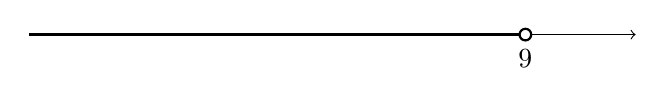
\begin{tikzpicture}[scale=0.7]
  \draw[->] (0,0) -- (11,0);
  \draw (9,0.1) -- (9,-0.1) node[below] {$9$};
  \draw[very thick] (0,0) -- (9,0); \abierto{9}
\end{tikzpicture}
\end{center}
\end{ejemplo}

\subsubsection*{Inecuaciones simultáneas}

Una doble desigualdad como $1 < -x + 1 < 5$ se resuelve operando las tres partes a
la vez: restando 1 queda $0 < -x < 4$, y al multiplicar por $-1$ se invierten
\emph{ambos} signos: $0 > x > -4$. Solución: $(-4, 0)$.

\begin{ejemplo}[Cuando no se puede despejar en el centro]
En $2 + 2x < x - 1 < 5$ la $x$ aparece en dos partes, así que se separa en dos
inecuaciones que deben cumplirse a la vez: $2 + 2x < x - 1$, que da $x < -3$, y
$x - 1 < 5$, que da $x < 6$. La solución es la intersección:
$(-\infty, -3) \cap (-\infty, 6) = (-\infty, -3)$.
\end{ejemplo}

\begin{aplicacion}[Elegir un plan de celular]
El plan A cuesta $\$20\,000$ al mes más $\$150$ por minuto; el plan B, $\$35\,000$
más $\$50$ por minuto. Con $m$ minutos, A es más barato cuando
$20\,000 + 150m < 35\,000 + 50m$, es decir, $100m < 15\,000$ y $m < 150$. Si hablas
menos de 150 minutos al mes, conviene A.
\end{aplicacion}

\begin{preguntas}
\pregunta Resuelve y escribe la solución como intervalo:
\begin{opciones*}(3)
  \item $5x + 2 \ge 3x - 6$
  \item $\dfrac{x - 1}{3} < 2 - x$
  \item $-4 \le 2x + 2 < 10$
\end{opciones*}
\espacio{4cm}
\pregunta Un estudiante tiene notas de $3{,}5$ y $4{,}2$ en dos quices. ¿Qué nota
necesita en el tercero para que el promedio de los tres sea al menos $4{,}0$?
\espacio{3cm}
\pregunta La ley de Ohm dice que la corriente es $I = \dfrac{V}{R}$ (en amperios),
donde $V$ es el voltaje y $R > 0$ la resistencia (en ohmios). Con $V = 110$ V,
¿qué resistencias producen una corriente de máximo 10 A?
\espacio{3cm}
\pregunta La fórmula $C = \frac{5}{9}(F - 32)$ convierte grados Fahrenheit en
Celsius. ¿Qué temperaturas en °F corresponden a menos de 30 °C?
\espacio{2.5cm}
\end{preguntas}

\begin{resumen}
\begin{itemize}
  \item Una inecuación se resuelve como una ecuación, con una excepción: al
        multiplicar o dividir por un negativo, se invierte el sentido.
  \item La solución es un conjunto (casi siempre un intervalo); se comprueba con
        un valor de adentro y uno de afuera.
  \item Una doble desigualdad $a \le mx + b < c$ se resuelve operando las tres partes a la vez.
\end{itemize}
\end{resumen}

% ---------------------------------------------------------------------
\tema{Inecuaciones cuadráticas y racionales}\label{tema:cuadraticas}

\begin{hilo}
Hacia el año 400, Hipatia explica en Alejandría los problemas de Diofanto. Algunos
llevan a cuadrados de la incógnita, y ya no basta con despejar: hay que estudiar
dónde una expresión es positiva y dónde negativa.
\end{hilo}

\subsubsection*{Método de la tabla de signos}
\begin{enumerate}[label=\arabic*.]
  \item Pasa todo a un lado: $P(x) > 0$, $P(x) \le 0$, etc.
  \item Factoriza y halla los \textbf{puntos críticos}: donde cada factor vale cero
        (y, en las racionales, donde el denominador vale cero).
  \item Divide la recta con esos puntos y estudia el signo de cada factor en cada tramo.
  \item Elige los tramos que cumplen la desigualdad. Los ceros del denominador
        \emph{nunca} se incluyen.
\end{enumerate}

\begin{ejemplo}[Cuadrática]
$x^2 - x - 6 \le 0 \;\Longleftrightarrow\; (x - 3)(x + 2) \le 0$. Puntos críticos:
$-2$ y $3$.
\begin{center}
{\renewcommand{\arraystretch}{1.3}
\begin{tabular}{c|ccc}
  & $(-\infty, -2)$ & $(-2, 3)$ & $(3, \infty)$\\\hline
  $x + 2$ & $-$ & $+$ & $+$\\
  $x - 3$ & $-$ & $-$ & $+$\\\hline
  producto & $+$ & $-$ & $+$\\
\end{tabular}}
\end{center}
Como pide $\le 0$: solución $[-2, 3]$ (los extremos se incluyen porque ahí el
producto vale 0).
\end{ejemplo}

\begin{ejemplo}[Racional]
$\dfrac{x - 1}{x + 2} \ge 0$. Puntos críticos: $1$ (numerador) y $-2$ (denominador).
El cociente es positivo en $(-\infty, -2)$ y en $(1, \infty)$, y vale cero en
$x = 1$. Solución: $(-\infty, -2) \cup [1, \infty)$; el $-2$ se excluye porque
anula el denominador.
\end{ejemplo}

\begin{aplicacion}[El tiempo en el aire]
Si se lanza un balón hacia arriba a $20$ m/s, su altura es aproximadamente
$h(t) = -5t^2 + 20t$ metros. ¿Cuándo está por encima de 15 m? Resolviendo
$-5t^2 + 20t > 15$ se llega a $(t - 1)(t - 3) < 0$, es decir, $1 < t < 3$:
durante 2 segundos. Así se calculan las ventanas de tiempo en deportes,
ingeniería o fuegos artificiales.
\end{aplicacion}

\begin{preguntas}
\pregunta Resuelve con tabla de signos:
\begin{opciones*}(3)
  \item $x^2 - 4x < 0$
  \item $x^2 + 2x - 8 \ge 0$
  \item $\dfrac{x + 3}{x - 2} < 0$
\end{opciones*}
\espacio{4.5cm}
\pregunta Para recorrer 100 km a velocidad constante $v$ (en km/h) se tarda
$t = \dfrac{100}{v}$ horas. ¿A qué velocidades se tarda como máximo 2 horas?
Plantea la inecuación y resuélvela.
\espacio{3cm}
\pregunta Pedro resolvió $\dfrac{2}{x} < 1$ así: «Multiplico ambos lados por $x$ y
queda $2 < x$. Solución: $(2, \infty)$». ¿Qué paso no es correcto y por qué? Halla
la solución correcta con tabla de signos.
\espacio{3.5cm}
\pregunta Resuelve $(x - 2)(x + 3)(x + 5) \le 0$ con una tabla de signos de tres factores.
\espacio{3cm}
\pregunta La concentración de un medicamento en la sangre, $t$ horas después de
tomarlo, es $c(t) = \dfrac{20t}{t^2 + 4}$ mg/L, y hace efecto cuando supera 4 mg/L.
¿Durante qué intervalo de tiempo hace efecto? (Pista: ¿por qué aquí sí se puede
multiplicar por el denominador sin cambiar el sentido?)
\espacio{3.5cm}
\end{preguntas}

\begin{resumen}
\begin{itemize}
  \item Se factoriza, se hallan los puntos críticos y se estudia el signo en cada tramo.
  \item Con $\le$ o $\ge$, los ceros del numerador se incluyen; los ceros del
        denominador nunca.
  \item La solución puede ser una unión de intervalos.
\end{itemize}
\end{resumen}

% ---------------------------------------------------------------------
\tema{Valor absoluto}\label{tema:valorabsoluto}

\begin{hilo}
París, 1804. «Monsieur Le Blanc» escribe a Gauss. Detrás del seudónimo está Sophie
Germain, que aprendió matemáticas sola, de noche, con los libros de su padre. Su
historia nos recuerda que en matemáticas lo que importa no es quién eres, sino qué
tan lejos llega tu razonamiento. Y medir qué tan lejos está algo es exactamente
lo que hace el valor absoluto.
\end{hilo}

\begin{definicion}[Valor absoluto]
\[
  \abs{x} = \begin{cases} x & \text{si } x \ge 0,\\ -x & \text{si } x < 0. \end{cases}
\]
Geométricamente, $\abs{x}$ es la \textbf{distancia} de $x$ a $0$, y $\abs{x - a}$ es
la distancia de $x$ a $a$.
\end{definicion}

Para $k > 0$:
\[
  \abs{x} = k \iff x = \pm k, \qquad
  \abs{x} < k \iff -k < x < k, \qquad
  \abs{x} > k \iff x < -k \ \text{o}\ x > k.
\]

\begin{ejemplo}[Ecuación e inecuación]
$\abs{x - 3} = 5 \iff x - 3 = 5$ o $x - 3 = -5 \iff x = 8$ o $x = -2$.

$\abs{2x + 1} < 7 \iff -7 < 2x + 1 < 7 \iff -8 < 2x < 6 \iff -4 < x < 3$.
Solución: $(-4, 3)$.
\end{ejemplo}

\begin{aplicacion}[Tolerancias en la fabricación]
Una pieza debe medir 10 mm con una tolerancia de $0{,}05$ mm. En lenguaje
matemático: $\abs{d - 10} \le 0{,}05$, es decir, $9{,}95 \le d \le 10{,}05$. Las
fábricas de celulares, carros o aviones aceptan o rechazan piezas con
inecuaciones como esta.
\end{aplicacion}

\begin{preguntas}
\pregunta Resuelve:
\begin{opciones*}(3)
  \item $\abs{3x - 6} = 9$
  \item $\abs{x + 2} \le 5$
  \item $\abs{4 - x} > 1$
\end{opciones*}
\espacio{4cm}
\pregunta Una balanza tiene un error máximo de $0{,}2$ kg. Si marca $62{,}5$ kg,
escribe con valor absoluto los posibles pesos reales $p$ y el intervalo que forman.
\espacio{2.5cm}
\pregunta Escribe cada enunciado como una desigualdad con valor absoluto:
\begin{opciones}
  \item El radio $r$ de una pieza no debe diferir de 1 cm en más de $0{,}1$ cm.
  \item La diferencia de edad entre dos hermanos, de $x$ y $y$ años, es de máximo 4 años.
  \item La distancia entre $a$ y $b$ en la recta real está entre 5 y 27 unidades.
\end{opciones}
\espacio{2.5cm}
\pregunta ¿Se puede resolver $x^2 < 16$ «sacando raíz a ambos lados» y concluir
$x < 4$? Explica usando que $\sqrt{x^2} = \abs{x}$ y da la solución correcta.
\espacio{3cm}
\pregunta Comprueba con varios valores de $m$ y $n$ la desigualdad triangular
$\abs{m + n} \le \abs{m} + \abs{n}$. ¿Para qué valores se cumple la igualdad?
\espacio{3cm}
\end{preguntas}

\begin{resumen}
\begin{itemize}
  \item $\abs{x - a}$ es la distancia entre $x$ y $a$ en la recta real.
  \item $\abs{x} < k$: los puntos \emph{cerca} de 0 (un intervalo);
        $\abs{x} > k$: los puntos \emph{lejos} de 0 (unión de dos intervalos).
  \item El valor absoluto modela errores, tolerancias y márgenes.
\end{itemize}
\end{resumen}

% ---------------------------------------------------------------------
% 5. Cierre del hilo conductor
% ---------------------------------------------------------------------
\seccion{Prepárate para Saber 11}

\begin{instrucciones}
Preguntas de selección múltiple con única respuesta, como las de la prueba Saber 11.
Resuélvelas en tu cuaderno y compara tus respuestas con las de tus compañeros.
Adaptadas de la sección «Prepárate para el ICFES» de~\cite{quintero}.
\end{instrucciones}

\begin{preguntas}
\pregunta Una empresa de acueducto cobra $y = 1\,000x + 14\,000$ pesos al mes por
$x$ metros cúbicos (para consumos menores de 40 m³), donde $\$14\,000$ es el cargo
fijo. Un usuario quiere pagar entre el doble y el triple del cargo fijo. Debe
consumir entre:
\begin{opciones*}(4)
  \item 14 y 28 m³
  \item 28 y 42 m³
  \item 14 y 42 m³
  \item 0 y 14 m³
\end{opciones*}
\pregunta Un balón se lanza hacia arriba y su altura es $h(t) = -5t^2 + 30t$ metros.
¿Durante qué intervalo de tiempo (en segundos) está a más de 40 m de altura?
\begin{opciones*}(4)
  \item $(2, 4)$
  \item $(1, 5)$
  \item $(0, 6)$
  \item $(4, 6)$
\end{opciones*}
\pregunta En un concierto hay boletas de $\$20\,000$ y de $\$25\,000$. Entraron
5\,000 personas y la boletería debe sumar al menos $\$120$ millones. ¿Cuántas
boletas de $\$20\,000$ se pudieron vender como máximo?
\begin{opciones*}(4)
  \item 500
  \item 1\,000
  \item 2\,000
  \item 4\,000
\end{opciones*}
\pregunta Una varilla debe medir 50 cm, con un error máximo de $0{,}2$ cm. ¿Qué
expresión describe las longitudes aceptables $x$?
\begin{opciones*}(4)
  \item $\abs{x + 50} \le 0{,}2$
  \item $\abs{x - 50} \le 0{,}2$
  \item $\abs{x - 0{,}2} \le 50$
  \item $\abs{x} \le 50{,}2$
\end{opciones*}
\end{preguntas}

\seccion{Cierre: el paraíso de Cantor}

Empezamos con los pitagóricos, seguros de que todo cabía en los números enteros, y
terminamos con una recta que no tiene huecos, en la que entre dos números
cualesquiera caben infinitos otros, y que es tan grande que ni siquiera se puede
numerar. Fue necesario el valor de Hipaso, la paciencia de Hipatia, la
terquedad de Sophie Germain, la precisión de Dedekind y la audacia de Cantor.
Sobre esa recta construiremos el resto del año: las funciones en el segundo
trimestre y el cálculo en el tercero.

% ---------------------------------------------------------------------
% 6. Evaluación (secciones institucionales)
% ---------------------------------------------------------------------
\matrizevaluacion
  {Distingue los sistemas numéricos, justifica que existen irracionales y
   explica la densidad de los reales.}
  {Resuelve inecuaciones lineales, cuadráticas, racionales y con valor absoluto,
   y expresa sus soluciones como intervalos.}
  {Revisa sus procedimientos y los de sus compañeros con argumentos, aceptando el
   error como parte del aprendizaje.}
  {Reconoce que la matemática se ha construido colectivamente y valora a quienes,
   como Sophie Germain, la hicieron a pesar de la exclusión.}

\autoevaluacion

\seguimientodocente

% ---------------------------------------------------------------------
% 7. Referencias
% ---------------------------------------------------------------------
\begin{referencias}
% verificado: https://bibcatalogo.uca.es/cgi-bin/koha/opac-detail.pl?biblionumber=603122 — Gredos 1994, trad. T. Calvo Martínez; pasaje pitagórico en Met. I.5, 985b23–26
\bibitem{aristoteles} Aristóteles (1994). \emph{Metafísica} (trad. T. Calvo
  Martínez; Biblioteca Clásica Gredos, 200), libro I, cap. 5. Madrid: Gredos.
% verificado: https://link.springer.com/book/10.1007/978-94-009-9051-7 — D. Reidel 1980; cap. 3 «Respectfully Yours, Gauss», pp. 20–29
\bibitem{bucciarelli} Bucciarelli, L. L. y Dworsky, N. (1980). \emph{Sophie
  Germain: An Essay in the History of the Theory of Elasticity}. Dordrecht:
  D. Reidel.
% verificado: https://www.math.ru.nl/werkgroepen/gmfw/bronnen/dedekind2.html — Vieweg 1872; el prólogo sitúa la idea en el otoño de 1858, en Zúrich (24 nov. 1858)
\bibitem{dedekind} Dedekind, R. (1872). \emph{Stetigkeit und irrationale
  Zahlen}. Braunschweig: Vieweg.
% verificado: https://www.hup.harvard.edu/books/9780674437760 — Harvard University Press, 1995
\bibitem{dzielska} Dzielska, M. (1995). \emph{Hypatia of Alexandria}.
  Cambridge, MA: Harvard University Press.
% verificado: https://link.springer.com/article/10.1007/BF01206605 — Mathematische Annalen 95 (1926), pp. 161–190
\bibitem{hilbert} Hilbert, D. (1926). Über das Unendliche. \emph{Mathematische
  Annalen}, 95, 161--190.
% verificado: https://global.oup.com/academic/product/mathematical-thought-from-ancient-to-modern-times-9780195014969 — Oxford University Press, 1972
\bibitem{kline} Kline, M. (1972). \emph{Mathematical Thought from Ancient to
  Modern Times}. Nueva York: Oxford University Press.
% verificado: https://gblumen.mineducacion.gov.co/cgi-bin/koha/opac-detail.pl?biblionumber=4785 — MEN 2016, ISBN 978-958-691-925-8
\bibitem{mendba} Ministerio de Educación Nacional (2016). \emph{Derechos
  Básicos de Aprendizaje V.2: Matemáticas}. Bogotá: MEN.
% verificado: recursos/matematicas/Guías pedagógicas Matemáticas/11 - Modulo_Matematicas_Undecimo.docx (archivo local) — autora y título tomados de la portada
\bibitem{quintero} Quintero Palomino, A. (s.\,f.). \emph{Conceptos de las funciones
  y las relaciones como introducción a grado 11.º} (Guía de apoyo educativo en el
  área de las matemáticas).
% verificado: https://www.cengage.com/c/ebook-prec%C3%A1lculo-matem%C3%A1ticas-para-el-c%C3%A1lculo-7e-stewart-redlin-watson/9780357087091/ — Cengage, 7.ª ed.
\bibitem{stewart} Stewart, J., Redlin, L. y Watson, S. (2017).
  \emph{Precálculo: matemáticas para el cálculo} (7.ª ed.). México: Cengage Learning.
\end{referencias}

\end{document}
